\documentclass{article}

\usepackage[utf8]{inputenc}
\usepackage[brazil]{babel}

\usepackage{Sweave}
\begin{document}
\Sconcordance{concordance:1703.tex:1703.Rnw:%
1 5 1 1 0 12 1 1 8 1 3 11 1 1 22 1 3 19 1 1 12 1 3 8 1}


\section{Aula 02}

%##################################

\subsection{Classificador univariado}
Teste de classificador univariado (figura \ref{fig:Fig1}).

\setkeys{Gin}{width=0.6\textwidth}
\begin{figure}[h]
\centering
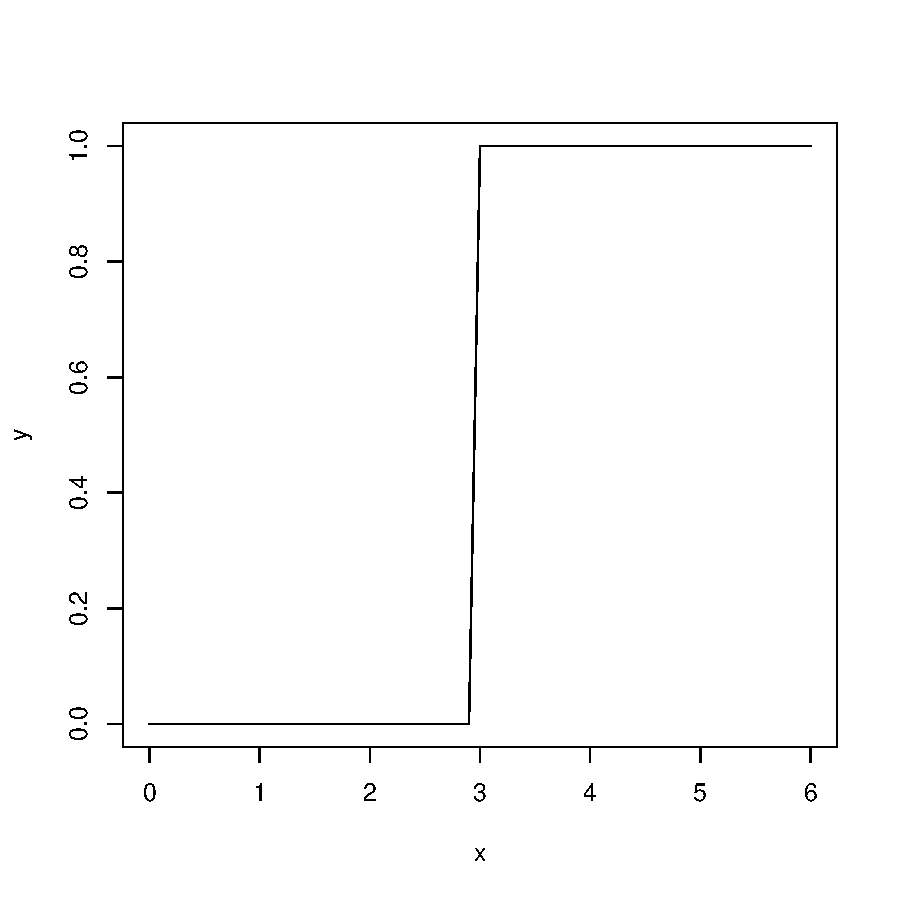
\includegraphics{1703-001}
\caption{Classificador univariado}
\label{fig:Fig1}
\end{figure}

%##################################

\subsection{Superfície 3D}
Teste de plot 3D (figura \ref{fig:Fig3}).

\setkeys{Gin}{width=0.6\textwidth}
\begin{figure}[!htb]
\centering
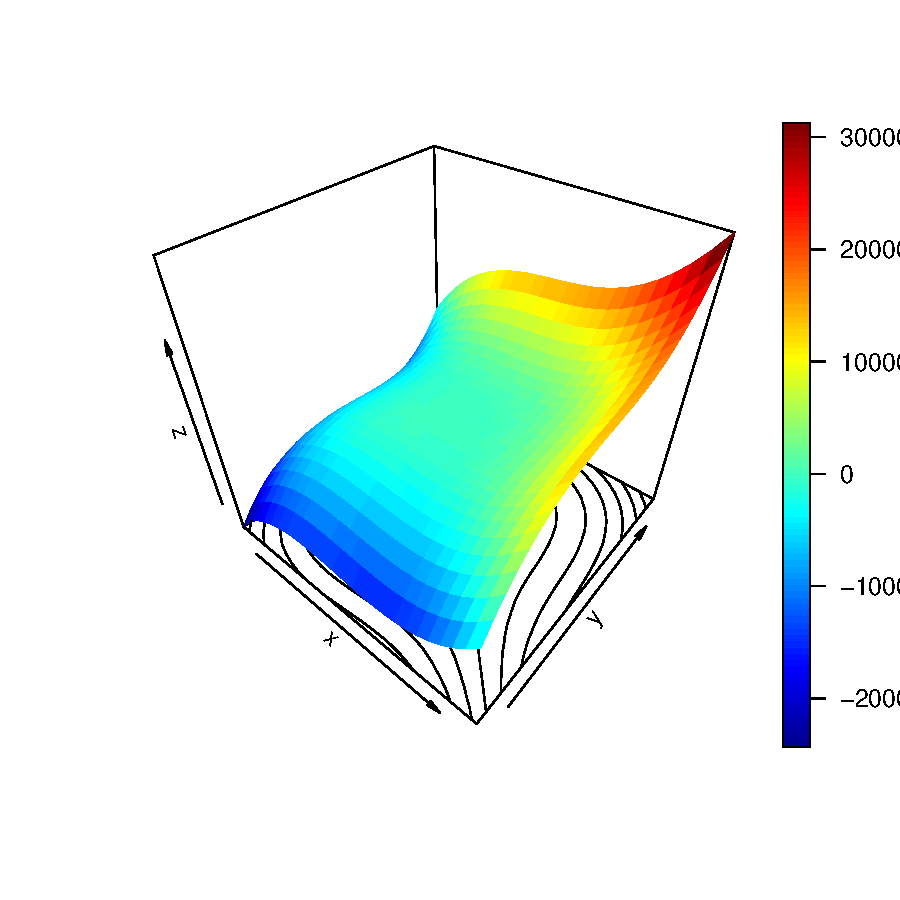
\includegraphics{1703-002}
\caption{Superfície 3D}
\label{fig:Fig3}
\end{figure}

%##################################

\subsection{Perceptron Simples}

Perceptron simples (moodle) (figura \ref{fig:Fig2}).

\begin{itemize}
\item Duas classes 
\item Distancia a reta x$_2$ + x$_1$ - 6 = 0
\item Pesos: w = [1,1,-6]$^T$
\item x = [x$_1$,x$_2$,1]$^T$
\end{itemize}

\setkeys{Gin}{width=0.6\textwidth}
\begin{figure}[!htb]
\centering
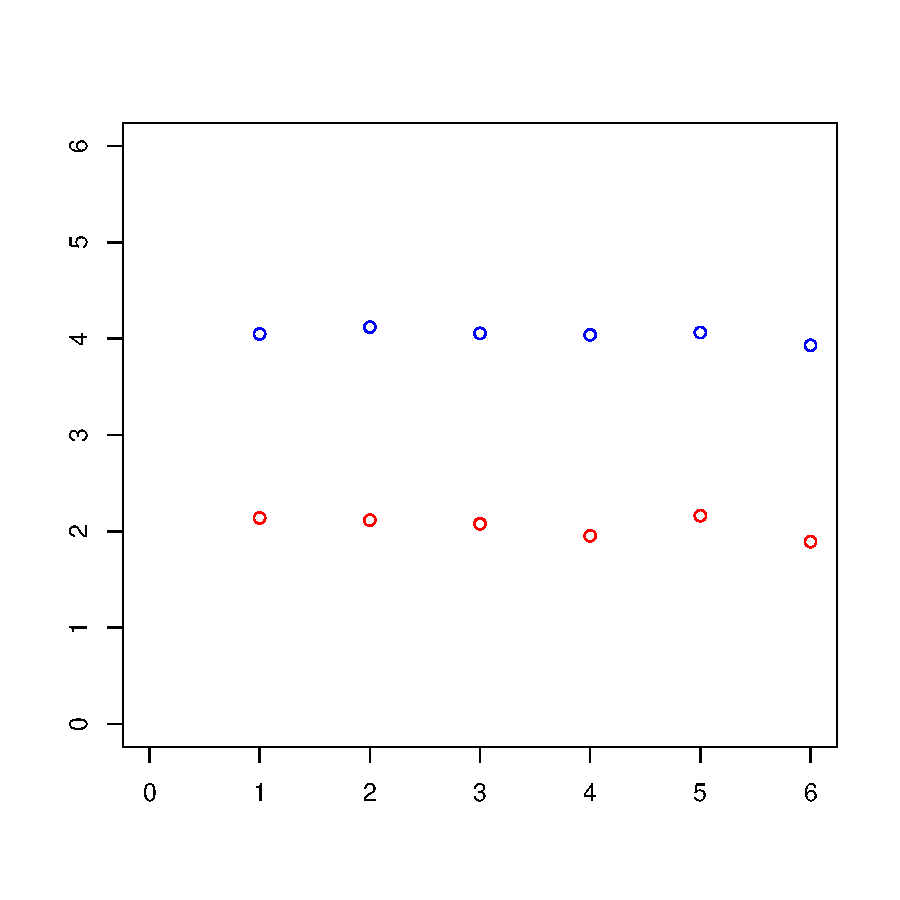
\includegraphics{1703-003}
\caption{Perceptron simples}
\label{fig:Fig2}
\end{figure}

(Figura aleatória, exercício incompleto)

%##################################

\end{document}
